% Rieke, Ken    4234782
% Thill, Gregor 4260617

\documentclass[12pt,a4paper,bibliography=totoc]{scrbook}
\usepackage[utf8]{inputenc}
\usepackage[T1]{fontenc}
\usepackage[ngerman]{babel}
\usepackage{graphicx}

\hyphenation{Col-le-gi-um}
\hyphenation{Ca-ro-li-num}

\begin{document}
\title{Ein Beispiel für ein größeres Projekt}
\author{Max Mustermann}
\date{12. Januar 2015}
\maketitle
\tableofcontents
\listoffigures

\chapter{Das erste Kapitel}

\section*{Einführung}
Dieser Text soll ihnen helfen, Latex zu lernen. Ob dies auch so funktioniert,
weiß ich natürlich nicht, Ich bin aber zuversichtlich.

Nun soll es ja heute um größere Projekte gehen. Dabei spielen vor allem viele
Details eine sehr große Rolle. So sollte die notwendige Trennung von besonders
langen und dabei extrem ungewöhnlichen Wörtern wie zum Beispiel das Wort
TU-Stu\-die\-ren\-den\-be\-ra\-tungs\-an\-ge\-bot möglichst gut klappen. Auch
sollte nichts überstehen, dies wäre sehr ungünstig für das Schriftbild.

Nun beginnt ein weiterer Absatz, obwohl dieser keinen sinnvollen Text mehr
enthält.

\section*{Überblick}
Der Text enthält ein weiteres Kapitel, in dem Sie zeigen sollen, wie Sie mit
Bildern und Literaturverweisen umgehen.

\chapter[Bilder]{Das Kapitel, dass die ganzen Bilder enthält und daher eine
lange Überschrift hat}

\section{Erstes Bild und Hinweise}
Hier geht es nun um ein tolles Bild. Schauen Sie das Bild \ref{fig:audimax_kippt}
auf dieser Seite an. Ob das so gut für das Audimax ist, bleibt zu bezweifeln.

Als nächstes benötigen wir einen Fülltext, in dem ich ihnen etwas zur Geschichte
der Universität mitteile. Dies können Sie ebenso in der Wikipedia nachlesen oder
einfach das Buch von Herrn Mummelhausen lesen, den Sie unter \cite{mummel} im
Literaturverzeichnis finden.

Dies ist übrigens der einzige Literaturverweis im Text. Auf die zweite Quelle im
Literaturverzeichnis gibt es keinen Verweis im Text. Außerdem sollten Sie den
passenden Stil für das Literaturverzeichnis wählen.

\section{Auszug aus der Geschichte der Uni}
Die heutige Technische Universität Braunschweig geht zurück auf eine
1745 auf Anregung des Hofpredigers J.~F.~W.~Jerusalem durch Carl~I. unter
dem Namen Collegium~Carolinum in Braunschweig gegründete Bildungsinstitution,
welche zwischen Gymnasium und
\begin{figure}
  \begin{center}
    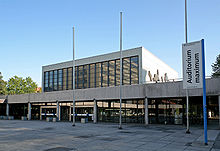
\includegraphics[width=4cm, angle=45]{audimax}
    \caption{Das Audimax kippt um}
    \label{fig:audimax_kippt}
  \end{center}
\end{figure}

\noindent Universität einzuordnen ist. Die Aufgabe des am Bohlweg angesiedelten
Collegium~Carolinum war zunächst vor allem die Ausbildung von Beamten. Mit der
Berufung von Literaturhistorikern wie Johann Joachim Eschenburg und dem Kreis
der Bremer Beiträger an das Collegium~Carolinum sowie Gotthold Ephraim Lessing
an die Herzog August Bibliothek wurde das Fürstentum Braunschweig-Wolfenbüttel
in der zweiten Hälfte des 18. Jahrhunderts für kurze Zeit zu einem
intellektuellen Zentrum der Aufklärung in Deutschland. Nach seiner Auflösung
im Jahre 1808 und der Umwandlung in eine Militärakademie wurde das Collegium
1814 wieder eröffnet. Nach einer immer stärkeren Zunahme der
naturwissenschaftlich-technischen Fächer wurde das Collegium 1878 in
Herzogliche Technische Hochschule Carolo-Wilhelmina umbenannt, und erhielt
schließlich 1968 den aktuellen Namen Technische Universität Carolo-Wilhelmina
zu Braunschweig.
\begin{figure}
  \begin{center}
    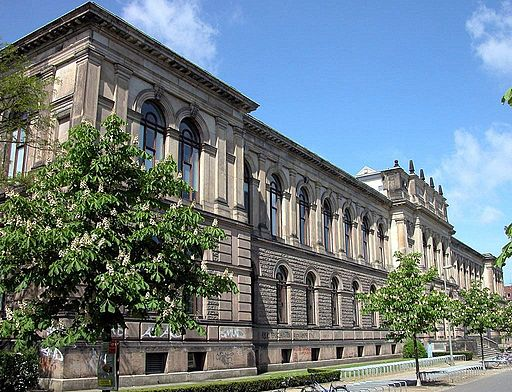
\includegraphics[width=2cm, height=10cm]{tu}
    \caption{Das Altgebäude mal ganz schlank}
    \label{fig:audimax_schlank}
  \end{center}
\end{figure}

\section{Ein weiteres Bild}
Auch auf dieser Seite finden Sie ein schönes Bild. Haben Sie es schon gefunden?

\bibliographystyle{alpha}
\bibliography{literatur}
\nocite{bilderbuch}
\end{document}
